\section{Introduction To The Problem}
The Minimum Height Problem an optimization problem relating to ladder lotteries.
Let the \emph{height} of a ladder be the number of rows that a ladder has. 
The Minimum Height Problem asks, given $OptL\{\pi\}$, what ladders in the set have the shortest height? 
Let $MinL\{\pi\} \subseteq OptL\{\pi\}$ such that the ladders in $MinL\{\pi\}$ are the shortest ladders from 
$OptL\{\pi\}$. Let \emph{a minimal ladder} be a ladder from $MinL\{\pi\}$. Given a permutation $\pi$, is there an algorithm for generating a minimal ladder
from $MinL\{\pi\}$?\par  
Some tangential questions that result from this problem are the following. Let $MinL\{\pi_{N}\}$ 
be the set of all $MinL\{\pi\}$ for each permutation of order $N$. Recall that $OptL\{\pi_{N}\}$ is the set of all 
$OptL\{\pi\}$ of order $N$. Thus, $MinL\{\pi_{N}\} \subseteq OptL\{\pi_{N}\}$.  The first tangential question is, 
what are the upper and lower bounds for a minimal ladder in $MinL\{\pi_{N}\}$? 
Let \emph{ladders of order N} pertain to ladders derived from some $\pi$ with $N$ elements.
The second tangential question is what ladders of order $N$ have a height of zero or one? 
Thirdly, is $|MinL\{\pi\}|=1$, or in other words is there 
only one ladder from $OptL\{\pi\}$ with a minimal height?\par 



Firstly I will address the tangential questions in the introduction. Following the tangential questions, 
I will provide a heuristic algorithm for generating one ladder from $MinL\{\pi\}$ in the procedures section. 
In the results section I will provide a table with the heights of the ladder from the heuristic algorithm in comparison to the heights of the ladders
in $MinL\{\pi\}$. Finally, in the analysis section there will be a discussion 
about the efficacy of the heuristic algorithm along with some applications of the algorithm.\par 


%%Upper and lower bounds question
\subsection{Upper and Lower Bounds of the heights of the Ladders in each $MinL\{\pi_{N}\}$}
In order to address the question as to what the upper and lower bounds for each $MinL\{\pi_{N}\}$ 
some points of clarification need to be addressed. It must be noted that each $MinL\{\pi_{N}\} \subseteq$ of each
corresponding $OptL\{\pi_{N}\}$. For example, let $N=4$, there are $24$ or $4!$ $OptL\{\pi\}$ in $OptL\{\pi_{4}\}$, which is to say 
each permutation of order $4$ has its own $OptL\{\pi\}$. Each $MinL\{\pi_{4}\}$ is a subset of one of the $24$
$OptL\{\pi_{4}\}$. We are going to determine what the upper and lower bounds for the heights of the ladders in $MinL\{\pi_{N}\}$ are;
not the upper and lower bounds for the heights of the ladders in $OptL\{\pi_{N}\}$. Although the lower bound for the 
height of a ladder in $MinL\{\pi_{N}\}$ will also be the lower bound for the height of a ladder in $OptL\{\pi_{N}\}$
seeing as the ladder from $MinL\{\pi_{N}\}$ that has the lower bound for its height will be the shortest ladder 
from all $OptL\{\pi_{N}\}$.
\begin{lemma}
    The lower bound for the height of a ladder $MinL\{\pi_{N}\}$ is zero
\end{lemma} 
\begin{proof}
    If $\pi_{N}$ is the sorted permutation of order $N$ then there are no 
    bars in its ladder. Recall that a bar swaps an adjacent inversion in $\pi$.
    Seeing as there are no adjacent inversions in the sorted permutation of 
    order $N$, then there are no bars that need to be added to its corresponding 
    ladder. Since a ladder with no bars requires no rows, then the lower 
    bound for the height of a ladder from $MinL{\pi_{N}}$ is zero. This is 
    the ladder belonging to $OptL\{\pi_{ID_{N}}\}$.
\end{proof}\par 
The upper bound for the heights of the ladders in $MinL\{\pi_{N}\}$ is more difficult to prove than the lower bound. 
The lower bound is unique seeing as there is only one ladder of order $N$ with zero bars. 
With the upper bound however, it has yet to be shown if there is an upper bound for 
$MinL\{\pi_{N}\}$. Before proving the upper bound for $MinL\{\pi_{N}\}$ it must be shown how to 
derive the ladder with minimal height from the root ladder of the reverse permutation of order $N$.
Once we have established how to derive the ladder with minimal height from the root ladder 
of the reverse permutation of order $N$, it will be relatively easy to prove the upper bound 
for $MinL\{\pi_{N}\}$.\par 
 Let $Degen_{\pi_{N}}$ be the reverse permutation of order 
 $N$. Let $MinL_{Degen_{\pi_{N}}}$ be a ladder with the shortest height for $Degen_{\pi_{N}}$.
 Let $R_{Degen}$ be the root ladder from $OptL_\{Degen_{\pi_{N}}\}$. Recall that the root ladder is the ladder such 
    that no bar of a lesser element has crossed the route of a greater element. $R_{degen}$ requires 
    $2(N-1)-1$ rows. The $Nth$ element requires $N-1$ rows seeing as each of the bars in its route cannot be on the same row as 
    any other bar in the same route. The route of the $Nth$ element spans from the first column to the $N-1th$ column.
    The $N-1th$ element requires $N-2$ bars. Seeing as the $N-1th$  element is directly to the right of the $Nth$ element 
    in $Degen_{\pi_{N}}$ and it requires $N-2$ bars in $R_{Degen}$; its firt bar in $R_{Degen}$ will be in the first column and its last bar will be in the
    $N-2th$ column. Since the endpoints of no two bars can be touching, the last bar of the $N-1th$ route 
    will be one row below the last bar of the $Nth$ route. The same pattern applies to the $N-2th$ element in relation 
    to the $N-1th$ element and so on. Since all the bars of a lesser route in $R_{Degen}$ must be below the route of 
    any greater element, this means the first bar of any route will begin at column one in the ladder. Since each bar 
    of the $N-Kth$, $0 \leq K < (N-1)$, element requires $N-K-1$ bars in its route, the route will span from column one to 
    column $N-K-1$; each bar of the route cannot share a row with any other bar in the route.
   Yet since the last bar of the previous element's route is at the currently lowest row in the ladder, a new row 
   will need to be added to the ladder to accomodate the last bar of the current element.\par 
   
   In order to create a ladder with minimal height from $OptL_\{Degen_{\pi_{N}}\}$, one simply needs to 
   take $R_{Degen}$ and modify it. In order to modify $R_{Degen}$ correctly, consider what happens when 
   the bars of lesser elements are swapped above the bars of greater elements. Of course, if this is done then 
   the ladder is no longer $R_{Degen}$. Nonetheless, when the $N-1th$ route is swapped above the $Nth$ route, 
   this frees up an extra row in the ladder for the $N-2th$ route. This is the row where the last bar of the $N-1th$ element resided
   before it was swapped above the $Nth$ route. Now, the first bar of the $N-1th$ route will begin in column $2$ and end at column $N-1$. 
   Furthermore, a new row will need to be added to the top of the ladder in order to accomodate the first bar of the $N-1th$ route. Now the route 
   of the $N-2th$ element can be raised up a row seeing as its last bar will still be in column $N-2$ and the row 
   that was previously occupied by the last bar of the $N-1th$ element will be free. Then the $N-3$ route can be swapped above 
   element $N$ and begin at column $4$ and span to column $N-1$. Since a new row was already added aboev route $N$ for element $N-1$
   and the first bar of element $N-1$ route began at column $2$, the first bar of element $N-3$ and go in the 
   same row as element $N-1$ seeing as the only other bar in this new row is at column 2. By  swapping 
   all the  $N-Jth$, $1 \leq J < (N-1)$ and $J=2K+1$, routes  above the route of the route of the $Nth$
   element in $R_{Degen}$, the ladder is reconfigured to have the minimal height. This height is $N$ because the 
   $Nth$ element still requires $N-1$ rows, and the $N-1th$ element will require a new row to be added above 
   the row of the first bar of the $Nth$ element to accomodate its first bar. Essentially, if $N$ is even, then 
   swap the route of each odd element in $R_{Degen}$ above route $N$ and keep the route of each even element below route $N$ 
   to create a ladder with $N$ rows. If $N$ is odd, then swap the route of each even element in $R_{Degen}$ above the 
   $Nth$ element and keep the route of eahc odd element below the route of $N$ to create a ladder with $N$ rows. Please refer 
   to figure --fig for an example of modifying $R_{5,4,3,2,1}$ to $MinL_{5,4,3,2,1}$.\pagebreak


   \begin{center}
        \begin{figure}[!htp]
            \begin{minipage}{.4\textwidth}
                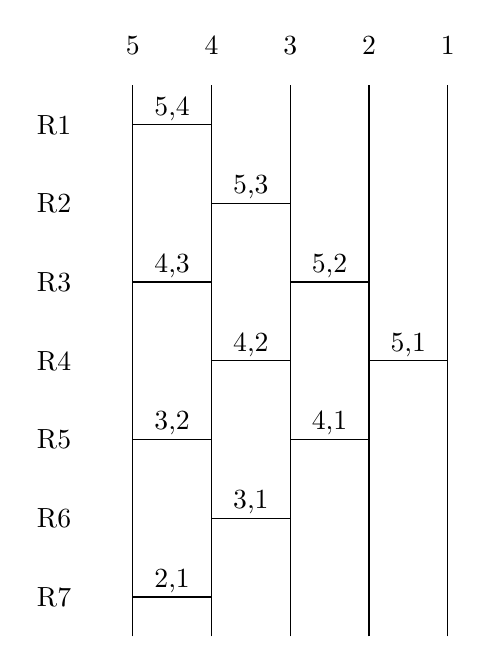
\begin{tikzpicture}
                    \draw(0, -1) to (0, 6);
                        %%draw the bars
                        \draw(0, 5.5) to (1, 5.5);
                            \node at (.5, 5.7){5,4};
                        \draw(0, 3.5) to (1, 3.5);
                            \node at (.5, 3.7){4,3};
                        \draw(0, 1.5) to (1, 1.5);
                            \node at (.5, 1.7){3,2};
                        \draw(0, -.5) to (1, -.5);
                            \node at (.5, -.3){2,1};
                    \draw(1, -1) to (1, 6);
                        \draw(1, 4.5) to (2, 4.5);
                            \node at(1.5, 4.7){5,3};
                        \draw(1, 2.5) to (2, 2.5);
                            \node at (1.5, 2.7){4,2};
                        \draw(1, .5) to (2, .5);
                            \node at(1.5, .7){3,1};
                    \draw(2, -1) to (2, 6);
                        \draw(2, 3.5) to (3, 3.5);
                            \node at(2.5, 3.7){5,2};
                        \draw(2, 1.5) to (3, 1.5);
                            \node at(2.5, 1.7){4,1};
                    \draw(3, -1) to (3, 6);
                        \draw(3, 2.5) to (4, 2.5);
                            \node at (3.5, 2.7){5,1};
                    \draw(4, -1) to (4, 6);

                    %%draw the rows
                    \node at (-1, 5.5){R1};
                    \node at(-1, 4.5){R2};
                    \node at(-1, 3.5){R3};
                    \node at (-1, 2.5){R4};
                    \node at(-1, 1.5){R5};
                    \node at (-1, 0.5){R6};
                    \node at (-1, -.5){R7};
                    %%draw the elements above the columns
                    \node at (0, 6.5){5};
                    \node at (1, 6.5){4};
                    \node at (2, 6.5){3};
                    \node at (3, 6.5){2};
                    \node at (4, 6.5){1};
                \end{tikzpicture}
            \end{minipage}
            \hfill
             \begin{minipage}{.4\textwidth}
                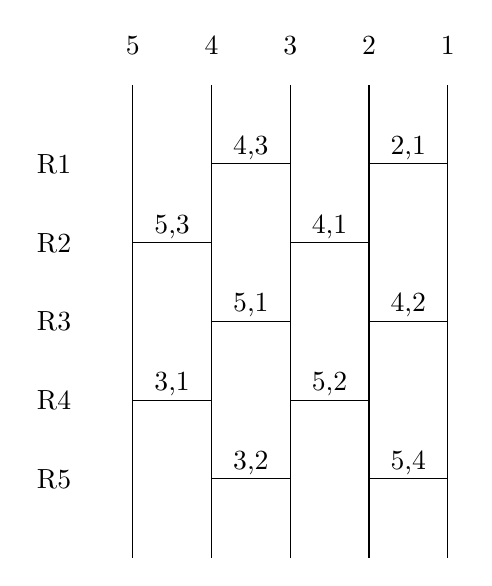
\begin{tikzpicture}
                    \draw(0, 0) to (0, 6);
                        \draw(0, 4) to (1, 4);
                            \node at(.5, 4.2){5,3};
                        \draw(0, 2) to (1, 2);
                            \node at(.5, 2.2){3,1};
                    \draw(1, 0) to (1, 6);
                        \draw(1, 3) to (2, 3);
                            \node at(1.5, 3.2){5,1};
                        \draw(1, 5) to (2, 5);
                            \node at(1.5, 5.2){4,3};
                        \draw(1, 1) to (2, 1);
                            \node at(1.5, 1.2){3,2};
                    \draw(2, 0) to (2, 6);
                        \draw(2, 2) to (3, 2);
                            \node at(2.5, 2.2){5,2};
                        \draw(2, 4) to (3, 4);
                            \node at(2.5, 4.2){4,1};
                    \draw(3, 0) to (3, 6);
                        \draw(3, 1) to (4, 1);
                            \node at(3.5, 1.2){5,4};
                        \draw(3, 3) to (4, 3);
                            \node at(3.5, 3.2){4,2};
                        \draw(3, 5) to (4, 5);
                            \node at(3.5, 5.2){2,1};
                    \draw(4, 0) to (4, 6);


                    %%nodes above
                    \node at (0, 6.5){5};
                    \node at (1, 6.5){4};
                    \node at (2, 6.5){3};
                    \node at (3, 6.5){2};
                    \node at (4, 6.5){1};

                    %%rows
                    \node at (-1, 5){R1};
                    \node at (-1, 4){R2};
                    \node at (-1, 3){R3};
                    \node at (-1, 2){R4};
                    \node at (-1, 1){R5};

                    %%nodes
    
                \end{tikzpicture}
            \end{minipage}
            \caption{The ladder to the left is $R_{5,4,3,2,1}$. The ladder to the left is $MinL_{5,4,3,2,1}$. Note that $N=5=2K+1$, thus 
            by swapping routes $2$ and $4$ above route $5$ whilst leaving route $3$ below route $5$ in $R_{5,4,3,2,1}$, we get 
            $MinL_{5,4,3,2,1}$. The height of $MinL_{5,4,3,2,1}$ is $5$. There is no way to reduce the height seeing as route $5$ still needs 
            $4$ rows and route $4$ needs one extra row for its first bar.}
        \end{figure}   

   \end{center}
   Now that $MinL_{Degen_{\pi_{N}}}$ has been established, we will go back to proving the upper bound for 
   $MinL\{\pi_{N}\}$. 
   \begin{lemma}
       The upper bound for $MinL\{\pi_{N}\}$ is $N$.
   \end{lemma}
   \begin{proof}
       We shall use a proof by contradiction. Suppose that the upper bound for the height of $MinL\{\pi_{N}\}$ was greater than $N$. (It cannot be less than $N$ because 
       we have already demonstrated that the minimal height of the ladder for the reverse permutation is $N$). Let $MinL_{Degen_{N}}$ be the 
       minimal ladder for the reverse permutation of order $N$. Refer to figure --fig for an example of $MinL_{5,4,3,2,1}$. It will be shown that for each 
       ladder of order $N$ can be created by deriving it from $MinL_{Degen_{N}}$.
       Recall that a bar simply univerts an inversion in a permutation. By removing bars from $MinL_{Degen_{N}}$, that is effectively removing 
       inversions from $Degen_{\pi_{N}}$. Of course, when a bar is removed from  $MinL_{Degen_{N}}$, the laddr ceases to be  $MinL_{Degen_{N}}$. 
       Let $K$ be the number of bars in the current state of the ladder, wth $MinL_{Degen_{N}}$, $K=(N(N-1))/2$. Fpr each subsequent 
       ladder, $0 \leq K < (N(N-1))/2$. Thus, to create the minimal ladders with  $K=((N(N-1))/2)-1$ bars , simply one of the correct bars from $MinL_{Degen_{N}}$. 
       Once all the minimal ladders with  $K=((N(N-1))/2)-1$ bars have been created, simply remove the correct bar from each of these ladders with 
        $K=(N(N-1))/2-1$ bars to get all minimal ladders with  $K=((N(N-1))/2)-2$ bars.
       This process continues until each minimal ladder of order $N$ has been created. Since bars are only being removed from the initial ladder which is $MinL_{Degen_{N}}$, no more rows 
       will be added to the ladder. Removing a bar does not necessarily remove a row, but removing a bar definitely does not add a row to the ladder. Earlier we stated that 
       the height of $MinL_{Degen_{N}}$ is $N$, and at the same time we stated that we could create a minimal ladder of order $N$ by deriving it from $MinL_{Degen_{N}}$ 
       through removing bars. Yet at the beginning of the proof, 
       we supposed the upper bound was greater than $N$ which contradicts the claim that by removing bars from  
       $MinL_{Degen_{N}}$ the height of  $MinL_{Degen_{N}}$ will not increase. Thus, the upper bound for $MinL_\{\pi_{N}\}$ is $N$. 
       Please refer to figure --fig for each ladder with minimal height generated derived from $MinL_{4,3,2,1}$. 

   \end{proof}\pagebreak

   \begin{center}
        \begin{figure}[!htp]
            %%L1
            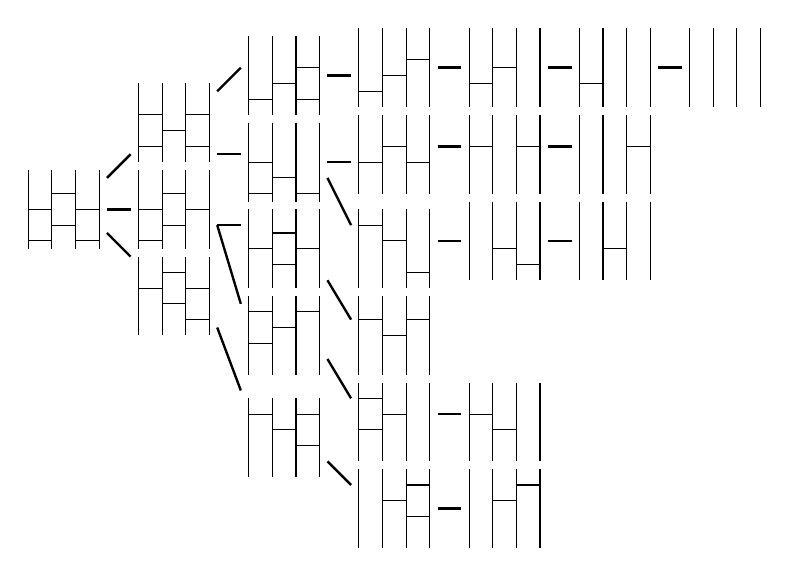
\begin{tikzpicture}
                \draw(0, -50) to (0, -51);
                    \draw(0, -50.5) to (.3, -50.5);
                    \draw(0, -50.9) to (.3, -50.9);
                \draw(0.3, -50) to (0.3, -51);
                    \draw(.3, -50.3) to (.6, -50.3);
                    \draw(.3, -50.7) to (.6, -50.7);
                \draw(0.6, -50) to (0.6, -51);
                    \draw(.6, -50.5) to (.9, -50.5);
                    \draw(.6, -50.9) to (.9, -50.9);
                \draw(0.9, -50) to (0.9, -51);
                
                \draw[line width = .3mm](1, -50.1) to (1.3, -49.8);
                \draw[line width = .3mm](1, -50.5) to (1.3, -50.5);
                \draw[line width = .3mm](1, -50.8) to (1.3, -51.1);
            
            %%L2
            \draw(1.4, -49.9) to (1.4, -48.9);
                \draw(1.4, -49.7) to (1.7, -49.7);
                \draw(1.4, -49.3) to (1.7, -49.3);
            \draw(1.7, -49.9) to (1.7, -48.9);
                \draw(1.7, -49.5) to (2, -49.5);
            \draw(2, -49.9) to (2, -48.9);
                \draw(2, -49.7) to (2.3, -49.7);
                \draw(2, -49.3) to (2.3, -49.3);
            
            \draw(2.3, -49.9) to (2.3, -48.9);
            %%L3
            \draw(1.4, -50) to (1.4, -51);
                \draw(1.4, -50.5) to (1.7, -50.5);
                \draw(1.4, -50.9) to (1.7, -50.9);
            \draw(1.7, -50) to (1.7, -51);
                \draw(1.7, -50.3) to (2, -50.3);
                \draw(1.7, -50.7) to (2, -50.7);
            \draw(2, -50) to (2, -51);
                \draw(2, -50.5) to (2.3, -50.5);
            \draw(2.3, -50) to (2.3, -51);

            %%L4
            \draw(1.4, -51.1) to (1.4, -52.1);
                \draw(1.4, -51.5) to (1.7, -51.5);
            \draw(1.7, -51.1) to (1.7, -52.1);
                \draw(1.7, -51.3) to (2, -51.3);
                \draw(1.7, -51.7) to (2, -51.7);
            \draw(2, -51.1) to (2, -52.1);
                \draw(2, -51.5) to (2.3, -51.5);
                \draw(2, -51.9) to (2.3, -51.9);
            \draw(2.3, -51.1) to (2.3, -52.1);

            \draw[line width=.3mm](2.4, -49) to (2.7, -48.7);
            \draw[line width=.3mm](2.4,-49.8) to (2.7, -49.8);
            \draw[line width=.3mm](2.4, -50.7) to (2.7, -50.7);
            \draw[line width=.3mm](2.4, -50.7) to (2.7, -51.7);
            \draw[line width = .3mm](2.4, -52) to (2.7, -52.8);

            %%L5
            \draw(2.8, -48.3) to (2.8, -49.3);
                \draw(2.8, -49.1) to (3.1, -49.1);
            \draw(3.1, -48.3) to (3.1, -49.3);
                \draw(3.1, -48.9) to (3.4, -48.9);
            \draw(3.4, -48.3) to (3.4, -49.3);
                \draw(3.4, -48.7) to (3.7, -48.7);
                \draw(3.4, -49.1) to (3.7, -49.1);
            \draw(3.7, -48.3) to (3.7, -49.3);

            %%L6
            \draw(2.8, -49.4) to (2.8, -50.4);
                \draw(2.8, -49.9) to (3.1, -49.9);
                \draw(2.8, -50.3) to (3.1, -50.3);
            \draw(3.1, -49.4) to (3.1, -50.4);
                \draw(3.1, -50.1) to (3.4, -50.1);
            \draw(3.4, -49.4) to (3.4, -50.4);
                \draw(3.4, -50.3) to (3.7, -50.3);
            \draw(3.7, -49.4) to (3.7, -50.4);

            %%L7
            \draw(2.8, -50.5) to (2.8, -51.5);
                \draw(2.8, -51) to (3.1, -51);
            \draw(3.1, -50.5) to (3.1, -51.5);
                \draw(3.1, -50.8) to (3.4, -50.8);
                \draw(3.1, -51.2) to (3.4, -51.2);
            \draw(3.4, -50.5) to (3.4, -51.5);
                \draw(3.4, -51) to (3.7, -51);
            \draw(3.7, -50.5) to (3.7, -51.5);
            %%L8
            \draw(2.8, -51.6) to (2.8, -52.6);
                \draw(2.8, -51.8) to (3.1, -51.8);
            \draw(3.1, -51.6) to (3.1, -52.6);
                \draw(3.1, -52) to (3.4, -52);
            \draw(3.4, -51.6) to (3.4, -52.6);
                \draw(3.4, -51.8) to (3.7, -51.8);
                \draw(2.8, -52.2) to (3.1, -52.2);
            \draw(3.7, -51.6) to (3.7, -52.6);
            
            %%L9
            \draw(2.8, -52.9) to (2.8, -53.9);
                \draw(2.8, -53.1) to (3.1, -53.1); 
            \draw(3.1, -52.9) to (3.1, -53.9);
                \draw(3.1, -53.3) to (3.4, -53.3);
            \draw(3.4, -52.9) to (3.4, -53.9);
                \draw(3.4, -53.1)to(3.7, -53.1);
                \draw(3.4, -53.5) to (3.7, -53.5);
            \draw(3.7, -52.9) to (3.7, -53.9);
            %%Lines
            \draw[line width = .3mm](3.8,-48.8) to (4.1,-48.8);
            \draw[line width = .3mm](3.8,-49.9) to (4.1,-49.9);
            \draw[line width = .3mm](3.8, -50.1) to (4.1, -50.7);
            \draw[line width = .3mm](3.8, -51.4) to (4.1, -51.9);
            \draw[line width = .3mm](3.8,-52.4) to (4.1,-52.9);
            \draw[line width = .3mm](3.8,-53.7) to (4.1,-54);

            %%L10
            \draw(4.2, -48.2) to (4.2, -49.2);
                \draw(4.2, -49) to (4.5, -49);
            \draw(4.5, -48.2) to (4.5, -49.2);
                \draw(4.5, -48.8) to (4.8, -48.8);
            \draw(4.8, -48.2) to (4.8, -49.2);
                \draw(4.8, -48.6) to (5.1, -48.6);
            \draw(5.1, -48.2) to (5.1, -49.2);

            %%L11
            \draw(4.2, -49.3) to (4.2, -50.3);
                \draw(4.2, -49.9) to (4.5, -49.9);
            \draw(4.5, -49.3) to (4.5, -50.3);
                \draw(4.5, -49.7) to (4.8, -49.7);
            \draw(4.8, -49.3) to (4.8, -50.3);
                \draw(4.8, -49.9) to (5.1, -49.9);
            \draw(5.1, -49.3) to (5.1, -50.3);
             %%L12
             \draw(4.2, -49.3) to (4.2, -50.3);
                \draw(4.2, -49.9) to (4.5, -49.9);
            \draw(4.5, -49.3) to (4.5, -50.3);
                \draw(4.5, -49.7) to (4.8, -49.7);
            \draw(4.8, -49.3) to (4.8, -50.3);
                \draw(4.8, -49.9) to (5.1, -49.9);
            \draw(5.1, -49.3) to (5.1, -50.3);

            %%L12
            \draw(4.2, -50.5) to (4.2, -51.5);
                \draw(4.2, -50.7) to (4.5, -50.7);
            \draw(4.5, -50.5) to (4.5, -51.5);
                \draw(4.5, -50.9) to (4.8, -50.9);
            \draw(4.8, -50.5) to (4.8, -51.5);
                \draw(4.8, -51.3) to (5.1, -51.3);
            \draw(5.1, -50.5) to (5.1, -51.5);

            %%L13
            \draw(4.2, -51.6) to (4.2, -52.6);
                \draw(4.2, -51.9) to (4.5, -51.9);
            \draw(4.5, -51.6) to (4.5, -52.6);
                \draw(4.5, -52.1) to (4.8, -52.1);
            \draw(4.8, -51.6) to (4.8, -52.6);
                \draw(4.8, -51.9) to (5.1, -51.9);
            \draw(5.1, -51.6) to (5.1, -52.6);

            %%L14
            \draw(4.2, -52.7) to (4.2, -53.7);
                \draw(4.2, -52.9) to (4.5, -52.9);
                \draw(4.2, -53.3) to (4.5, -53.3);
            \draw(4.5, -52.7) to (4.5, -53.7);
                \draw(4.5, -53.1) to (4.8, -53.1);
            \draw(4.8, -52.7) to (4.8, -53.7);
            \draw(5.1, -52.7) to (5.1, -53.7);

            %%L15
             \draw(4.2, -53.8) to (4.2, -54.8);
            \draw(4.5, -53.8) to (4.5, -54.8);
                \draw(4.5, -54.2) to (4.8, -54.2);
            \draw(4.8, -53.8) to (4.8, -54.8);
                \draw(4.8, -54) to (5.1, -54);
                \draw(4.8, -54.4) to (5.1, -54.4);
            \draw(5.1, -53.8) to (5.1, -54.8);

            %%Lines
            \draw[line width = .3mm](5.2, -48.7) to (5.5, -48.7);
            \draw[line width = .3mm](5.2, -49.7) to (5.5, -49.7);
            \draw[line width = .3mm](5.2, -50.9) to (5.5, -50.9);
            \draw[line width = .3mm](5.2, -53.1) to (5.5, -53.1);
            \draw[line width = .3mm](5.2, -54.3) to (5.5, -54.3);

            %%Ladders
            %%l16
            \draw(5.6, -48.2) to (5.6, -49.2);
                \draw(5.6, -48.9) to (5.9, -48.9);
            \draw(5.9, -48.2) to (5.9,  -49.2);
                \draw(5.9, -48.7) to (6.2, -48.7);
            \draw(6.2, -48.2) to (6.2,  -49.2);
            \draw(6.5, -48.2) to (6.5,  -49.2);
            %%l17
            \draw(5.6, -49.3) to (5.6, -50.3);
                \draw(5.6, -49.7) to (5.9, -49.7);
            \draw(5.9, -49.3) to (5.9, -50.3);
            \draw(6.2, -49.3) to (6.2, -50.3);
                \draw(6.2, -49.7) to (6.5, -49.7);
           \draw(6.5, -49.3) to (6.5, -50.3);

            %%l18
            \draw(5.6, -50.4) to (5.6, -51.4);
            \draw(5.9, -50.4) to (5.9, -51.4);
                \draw(5.9, -51) to (6.2, -51);
            \draw(6.2, -50.4) to (6.2, -51.4);
                \draw(6.2, -51.2) to (6.5, -51.2);
            \draw(6.5, -50.4) to (6.5, -51.4);

            %%l19
            \draw(5.6, -52.7) to (5.6, -53.7);
                \draw(5.6, -53.1) to (5.9, -53.1);
            \draw(5.9, -52.7) to (5.9, -53.7);
                \draw(5.9, -53.3) to (6.2, -53.3);
            \draw(6.2, -52.7) to (6.2, -53.7);
            \draw(6.5, -52.7) to (6.5, -53.7);

            %l20
            \draw(5.6, -53.8) to (5.6, -54.8);
            \draw(5.9, -53.8) to (5.9, -54.8);
                \draw(5.9, -54.2) to (6.2, -54.2);
            \draw(6.2, -53.8) to (6.2, -54.8);
                \draw(6.2, -54) to (6.5, -54);
            \draw(6.5, -53.8) to (6.5,-54.8);

            %%Lines
            \draw[line width = .3mm](6.6, -48.7) to (6.9, -48.7);
            \draw[line width = .3mm](6.6, -49.7) to (6.9, -49.7);
            \draw[line width = .3mm](6.6, -50.9) to (6.9, -50.9);


             %%l21
            \draw(7, -48.2) to (7, -49.2);
                \draw(7, -48.9) to (7.3, -48.9);
            \draw(7.3, -48.2) to (7.3,  -49.2);
            \draw(7.6, -48.2) to (7.6,  -49.2);
            \draw(7.9, -48.2) to (7.9,  -49.2);
            %%l22
            \draw(7, -49.3) to (7, -50.3);
            \draw(7.3, -49.3) to (7.3, -50.3);
            \draw(7.6, -49.3) to (7.6, -50.3);
                \draw(7.6, -49.7) to (7.9, -49.7);
           \draw(7.9, -49.3) to (7.9, -50.3);

            %%l23
            \draw(7, -50.4) to (7, -51.4);
            \draw(7.3, -50.4) to (7.3, -51.4);
                \draw(7.3, -51) to (7.6, -51);
            \draw(7.6, -50.4) to (7.6, -51.4);
            \draw(7.9, -50.4) to (7.9, -51.4);

            \draw[line width = .3mm](8, -48.7) to (8.3, -48.7);
             \draw(8.4, -48.2) to (8.4, -49.2);
             \draw(8.7, -48.2) to (8.7, -49.2);
             \draw(9, -48.2) to (9, -49.2);
             \draw(9.3, -48.2) to (9.3, -49.2);
        \end{tikzpicture}
        \end{figure}
   \end{center}
   %%End upper and lower bounds section


   %%Ladders with a height of zero or one section
   \subsection{Minimal Ladders of Order $N$ with Heights of Zero or One}
   There are some ladders of order $N$ which have a height of zero or one.
   There is only one permutation of order $N$ which results in a minimal ladder with a height of zero, 
   namely the identity permutation. This point has already been proven in the lemma for the lower bound of the 
   minimal height. What is more interesting is ladders of order $N$ with a height of one. 
   One may be tempted to assume that if the identity permutation results in a minimal ladder 
   with a height of zero, then all permutations of order $N$ with exactly one inversion result in minimal ladders with a height of one.
   Although this is true, it is only partially true. There are more permutations of order $N$ with more than one inversion 
   which result in minimal ladders with a height of one. Below will be presented one algorithm, one recurrence relation and one formula pertaining 
   to ladders of order $N$ with a height of one. The algrithm lists all ladders of order $N$ with a height of one. The recurrence relation
   counts all ladders of order $N$ with a height. The formula is the closed 
   form solution to the recurrence relation. The similarities between ladders of order $N$ with a height of one and other mathematical 
   objects will close off the topic.\par 

   \subsubsection{Listing Algorithm for all Ladders of Order $N$ with a Height of One}
   \begin{algorithm}
        \caption{Listing Algorithm For All Ladders of Order $N$ with a height of $1$}
        \begin{algorithmic}[1]
            \Function{GenHeightOne}{$Ladder[1][K=N-1]$, $Col=N-1$}
                \If{$Col<1$}
                    \State return
                \EndIf
                \State Ladder[1][$Col$] $\gets$ $1$
                \State $GENHEIGHTONE(Ladder, Col-2)$
                \State Ladder[1][$Col$] $\gets$ $0$
                \State $GENHEIGHTONE(Ladder, Col-1)$


            \EndFunction
        \end{algorithmic}    
   \end{algorithm}

   Let $Ladder$ be a two dimensional array initialized as the identity ladder of order $N$. Let $Col$ be initialized to $N-1$ indiciating the 
   current column. When a $1$ is inserted at $Ladder[1][Col]$ that indicates a bar has been added to row $1$, $Col$. When a $0$ is 
   inserted at $Ladder[1][Col]$ that indicates a bar has been removed from row $1$, $Col$. Since no two endpoints of two bars can be touching, 
   the function moves two columns to the 
   left on the first recursive call. This ensures that the next bar added will be two columns away from the current bar that was just added. 
   Once the $Col$ is less than $1$ the function returns to the previous value of $Col$ and removes the bar that was at $Ladder[1][Col]$. 
   This now frees the column that is one away from the  value of $Col$. Thus, the function makes a second recursive call, this time reducing $Col$ by one. 
   Each call to the function produces a unique ladder. To see the tree of all ladders with a height of one for $N=5$ please refer to figure --Fig\pagebreak

   \begin{figure}[!htp]
        \begin{center}
            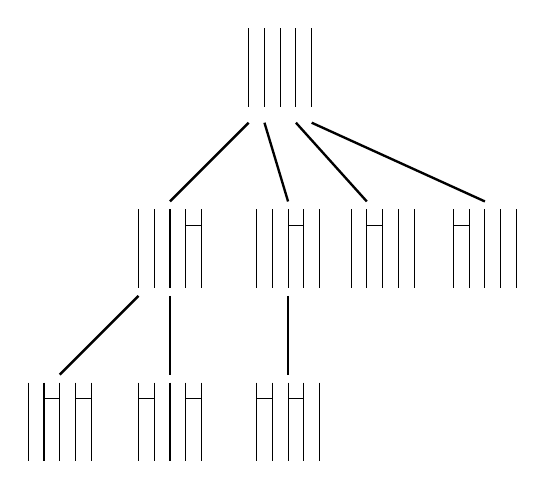
\begin{tikzpicture}
                \draw(0, 0) to (0, 1);
                \draw(.2, 0) to (.2, 1);
                \draw(.4, 0) to (.4, 1);
                \draw(.6, 0) to (.6, 1);
                \draw(.8, 0) to (.8, 1);

                \draw[line width = .3mm](0, -0.2) to (-1, -1.2);

                \draw[line width = .3mm](.2, -.2) to (.5, -1.2);

                \draw[line width = .3mm](.6, -.2) to (1.5, -1.2);
                \draw[line width = .3mm](.8, -.2) to (3, -1.2);

                \draw(-1.4, -1.3) to(-1.4, -2.3);
                \draw(-1.2, -1.3) to(-1.2, -2.3);
                \draw(-1, -1.3) to(-1, -2.3);
                \draw(-.8, -1.3) to(-.8, -2.3);
                    \draw(-.8, -1.5) to (-.6, -1.5);
                \draw(-.6, -1.3) to(-.6, -2.3);

                \draw(.1, -1.3) to (.1, -2.3);
                \draw(.3, -1.3) to (.3, -2.3);
                \draw(.5, -1.3) to (.5, -2.3);
                    \draw(.5, -1.5) to (.7, -1.5);
                \draw(.7, -1.3) to (.7, -2.3);
                \draw(.9, -1.3) to (.9, -2.3);

                \draw(1.3, -1.3) to (1.3, -2.3);
                \draw(1.5, -1.3) to (1.5, -2.3);
                    \draw(1.5, -1.5) to (1.7, -1.5);
                \draw(1.7, -1.3) to (1.7, -2.3);
                \draw(1.9, -1.3) to (1.9, -2.3);
                \draw(2.1, -1.3) to (2.1, -2.3);

                \draw(2.6, -1.3) to (2.6, -2.3);
                    \draw(2.6, -1.5) to (2.8, -1.5);
                \draw(2.8, -1.3) to (2.8, -2.3);
                \draw(3, -1.3) to (3, -2.3);
                \draw(3.2, -1.3) to (3.2, -2.3);
                \draw(3.4, -1.3) to (3.4, -2.3);

                \draw[line width = .3mm](-1.4, -2.4) to (-2.4, -3.4);
                \draw[line width = .3mm](-1, -2.4) to (-1, -3.4);
                \draw[line width = .3mm](.5, -2.4) to (.5, -3.4);
                
                \draw(-2.8, -3.5) to (-2.8, -4.5);
                \draw(-2.6, -3.5) to (-2.6, -4.5);
                    \draw(-2.6, -3.7) to (-2.4, -3.7);
                \draw(-2.4, -3.5) to (-2.4, -4.5);
                \draw(-2.2, -3.5) to (-2.2, -4.5);
                    \draw(-2.2, -3.7) to (-2, -3.7);
                \draw(-2, -3.5) to (-2, -4.5);

                \draw(-1.4, -3.5) to (-1.4, -4.5);
                    \draw(-1.4, -3.7) to (-1.2, -3.7);
                \draw(-1.2, -3.5) to (-1.2, -4.5);
                \draw(-1, -3.5) to (-1, -4.5);
                \draw(-.8, -3.5) to (-.8, -4.5);
                    \draw(-.8, -3.7) to (-.6, -3.7);
                \draw(-.6, -3.5) to (-.6, -4.5);

                 \draw(.1, -3.5) to (.1, -4.5);
                    \draw(.1, -3.7) to (.3, -3.7);
                \draw(.3, -3.5) to (.3, -4.5);
                \draw(.5, -3.5) to (.5, -4.5);
                   \draw(.5, -3.7) to (.7, -3.7);

                \draw(.7, -3.5) to (.7, -4.5);
                \draw(.9, -3.5) to (.9, -4.5);
            \end{tikzpicture}
        \end{center}
        \caption{All $7$ ladders of order $5$ with a height of one listed by the function $GenHeightOne$}
   \end{figure}

   \subsubsection{Recurrence Relation for Counting the Number of Ladders of Order $N$ with a Height of One}
   Although it may seem redunant to provide a recurrence relation to count the number of ladders of order $N$ with a height of one, seeing as 
   there is already an algorithm for listing all ladders of order $N$ with a height of one, one can use the recurrence relation to prove the 
   veracity of the listing algorithm. Also, the recurrence relation of the number of ladders of order $N$ is the same recurrence relation for 
   other combinatorial objects such as the number of involutions in the Symmetric Group $S_{N-1}$ or the number of permutations, $\pi$, of {1, 2, ..., n - 1} 
   such that $max|\pi_{i} - i| = 1$.\par 
   
   \begin{theorem}
       The recurrence relation for the number of ladders of order $N$ with a height of $1$ is:
       \[   \left\{
        \begin{array}{ll}
        L(0) = 0 & N = 0 \\
        L(1) = 0 & N=1 \\
        L(N) = L(N-1) + L(N-2) + 1 & N \geq 2 
        \end{array} 
    \right. \]
   \end{theorem}
\begin{proof}
    We shall do a combinatoial proof to demonstrate the above theorem. Suppose we want to count all binary strings of length $N$ such that there 
    can be no consecutive $1s$ and there must be at least one $1$ in the string. Suppose we are counting $1s$ from right to left. Suppose the first $1$ in a binary string of length $N$ is at position $N$, 
    then the second $1$ can appear at position $N-2$, thus we have binary 
    strings of length $N$ with the first $1$ appearing at position $N$ and the second one appearing at position $N-2$; let $M=$ the number of binary strings of length $N$ such that there is a $1$ 
    at position $N-2$. Suppose a binary string of length $N$ has a $0$ at position $N$, then
    the first $1$ can appear at position $N-1$ or position $N-2$. If it appears at position $N-2$ we have binary strings of length $N$ with a $1$ at position $N-2$. 
    We already designated this number as $M$, so we get $2(M)$. 
    Still supposing we are considering binary strings of length $N$ with a $0$ at position $N$, consider all binary strings of length $N-1$ with 
    no consecutive $1s$. Let $K=$ the number of binary strings of length $N-1$ with no consecutive $1s$ and at least one $1$.
    Let the first $1$ in the binary string of length $N$ appears at postion $N-1$, then we have $2(M)+K$. Still assuming a $0$ at position $N$
    in binary strings of length $N$, if there is also a $0$ at position $N-1$, then the first $1$ can appear at position $N-2$. The number of 
    binary strings of length $N$ with a $1$ at position $N$ was designated as $M$. Thus we have $2(M)+M=3M$
    Yet we have already counted $M$ under the conditions that the first $1$ in binary strings of length $N$ appears at position $N-2$. Therefore we subtract 
    $M$ from $K$ thus leaving us with $J=$ the number of binary strings of length $N$ with the first $1$ appearing at position $N-1$. 
    Now we have $2(M)+J$. Then consider all binary strings of length $N$ such that from positions $1\dots N-1$ there are 
    only $0s$. Therefore there must be a $1$ at position $N$ seeing as we are considering all binary strings of length $N$ with at least one $1$. 
    Since only one such binary string of length $N$ exists we simply add one. Thus we get $2(M)+(K-M)+1=2(M)+J+1=$ the number of binary strings of length $N$ with at least one $1$ and 
    no consecutive $1s$.\par 
    Now consder a ladder, $L$, with $N+1$ lines. The number of columns in $L$ is $N$. The stipulation of $L$ is that $L$ has a height of one. Note that the end points 
    of no two bars can be touching which is to say that there can be no adjacent bars on the same row. For example, if there is a bar at row $1$, column $N$ then 
    the next consecutive bar in row $1$ can appear at most at column $N-2$. Knowing this, we can easily see how this scenario models all binary strings of length $N$ with no 
    consecutive $1s$ and having at least one $1$. Let a bar in $L$ be represented as a $1$ in a binary string of length $N$. 
    Knowing that a ladder with zero bars has a height of zero, it must be the case that $L$ has at least one bar. Thus we get the same formula for the number of 
    ladders of order $N+1$ where $M$ is the number of ladders with a bar appearing in column $N-2$, $(K-M)=J$ being the number of ladders with the first bar in column $N-1$ minus 
    all ladders with the first bar appearing at column $N-2$. Lastly is the $+1$ for all ladders of order $N+1$ where the only bar appears at column $N$.
    See figure --Fig for the mapping of binary strings of length $N=5$ with no consecutive $1s$ and at least one $1$ to ladders of order $6$ with a height of one.\pagebreak

\end{proof}

\begin{center}
    
\begin{figure}[!htp]
    \begin{minipage}{.4\textwidth}

    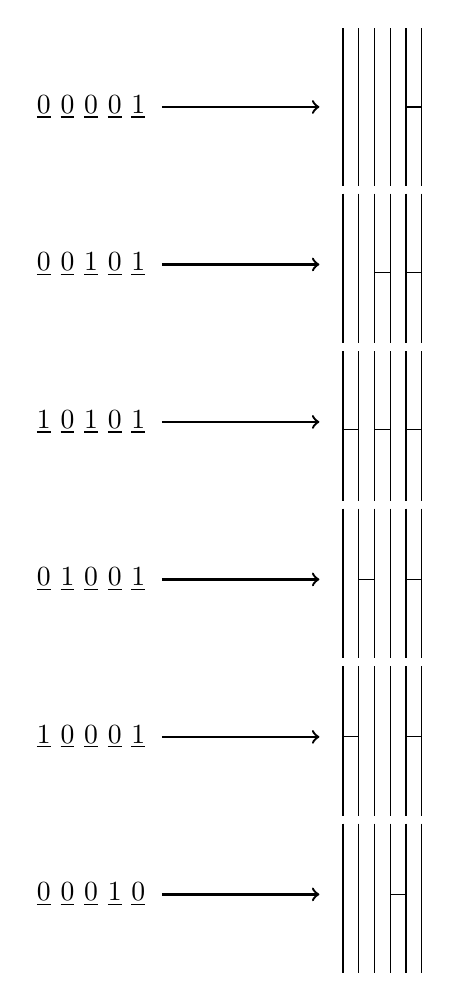
\begin{tikzpicture}
            
        
            
        %%B1
        \node at(0, 0){\underline{$0$}};
        \node at(0.3, 0){\underline{$0$}};
        \node at(0.6, 0){\underline{$0$}};
        \node at(0.9, 0){\underline{$0$}};
        \node at(1.2, 0){\underline{$1$}};
            \draw[->, line width = .3mm](1.5, 0) to (3.5, 0);
        %%L1
        \draw(3.8, -1) to (3.8, 1);
        \draw(4, -1) to (4, 1);
        \draw(4.2, -1) to (4.2, 1);
        \draw(4.4, -1) to (4.4, 1);
            \draw(4.6, 0) to (4.8, 0);
        \draw(4.6, -1) to (4.6, 1);
        \draw(4.8, -1) to (4.8, 1);
        %B2
        \node at (0, -2){\underline{$0$}};
        \node at (.3, -2){\underline{$0$}};
        \node at (.6, -2){\underline{$1$}};
        \node at (.9, -2){\underline{$0$}};
        \node at (1.2, -2){\underline{$1$}};
            \draw[->, line width = .3mm](1.5, -2) to (3.5, -2);

        %%L2
        \draw(3.8, -1.1) to (3.8, -3);
        \draw(4, -1.1) to (4, -3);
        \draw(4.2, -1.1) to (4.2, -3);
        \draw(4.4, -1.1) to (4.4, -3);
            \draw(4.6, -2.1) to (4.8, -2.1);
            \draw(4.2, -2.1) to (4.4, -2.1);
        \draw(4.6, -1.1) to (4.6, -3);
        \draw(4.8, -1.1) to (4.8, -3);

        %%B3
        \node at (0, -4){\underline{$1$}};
        \node at (.3, -4){\underline{$0$}};
        \node at (.6, -4){\underline{$1$}};
        \node at (.9, -4){\underline{$0$}};
        \node at (1.2, -4){\underline{$1$}};
                    \draw[->, line width = .3mm](1.5, -4) to (3.5, -4);

        %%L3
        \draw(3.8, -3.1) to (3.8, -5);
        \draw(4, -3.1) to (4, -5);
        \draw(4.2, -3.1) to (4.2, -5);
        \draw(4.4, -3.1) to (4.4, -5);
            \draw(4.6, -4.1) to (4.8, -4.1);
            \draw(4.2, -4.1) to (4.4, -4.1);
            \draw(3.8, -4.1) to (4, -4.1);
        \draw(4.6, -3.1) to (4.6, -5);
        \draw(4.8, -3.1) to (4.8, -5);
    
        %%B4
        \node at (0, -6){\underline{$0$}};
        \node at (.3, -6){\underline{$1$}};
        \node at (.6, -6){\underline{$0$}};
        \node at (.9, -6){\underline{$0$}};
        \node at (1.2, -6){\underline{$1$}};

        \draw[->, line width=.3mm](1.5, -6) to (3.5, -6);
        %%L4
        \draw(3.8, -5.1) to (3.8, -7);
        \draw(4, -5.1) to (4, -7);
            \draw(4, -6) to (4.2, -6);
        \draw(4.2, -5.1) to (4.2, -7);
        \draw(4.4, -5.1) to (4.4, -7);
        \draw(4.6, -5.1) to (4.6, -7);
            \draw(4.6, -6) to (4.8, -6);
        \draw(4.8, -5.1) to (4.8, -7);

        %%B5
        \node at (0, -8){\underline{$1$}};
        \node at (.3, -8){\underline{$0$}};
        \node at (.6, -8){\underline{$0$}};
        \node at (.9, -8){\underline{$0$}};
        \node at (1.2, -8){\underline{$1$}};

            \draw[->, line width=.3mm](1.5, -8) to (3.5, -8);
        %%L5
        \draw(3.8, -7.1) to (3.8, -9);
        \draw(4, -7.1) to (4, -9);
            \draw(3.8, -8) to (4, -8);
        \draw(4.2, -7.1) to (4.2, -9);
        \draw(4.4, -7.1) to (4.4, -9);
        \draw(4.6, -7.1) to (4.6, -9);
            \draw(4.6, -8) to (4.8, -8);
        \draw(4.8, -7.1) to (4.8, -9);

         %%B6
        \node at (0, -10){\underline{$0$}};
        \node at (.3, -10){\underline{$0$}};
        \node at (.6, -10){\underline{$0$}};
        \node at (.9, -10){\underline{$1$}};
        \node at (1.2, -10){\underline{$0$}};

            \draw[->, line width=.3mm](1.5, -10) to (3.5, -10);
        %%L6
        \draw(3.8, -9.1) to (3.8, -11);
        \draw(4, -9.1) to (4, -11);
        \draw(4.2, -9.1) to (4.2, -11);
        \draw(4.4, -9.1) to (4.4, -11);
            \draw(4.4, -10) to (4.6, -10);
        \draw(4.6, -9.1) to (4.6, -11);
        \draw(4.8, -9.1) to (4.8, -11);

    \end{tikzpicture}
    \end{minipage}
    \begin{minipage}{.4\textwidth}
        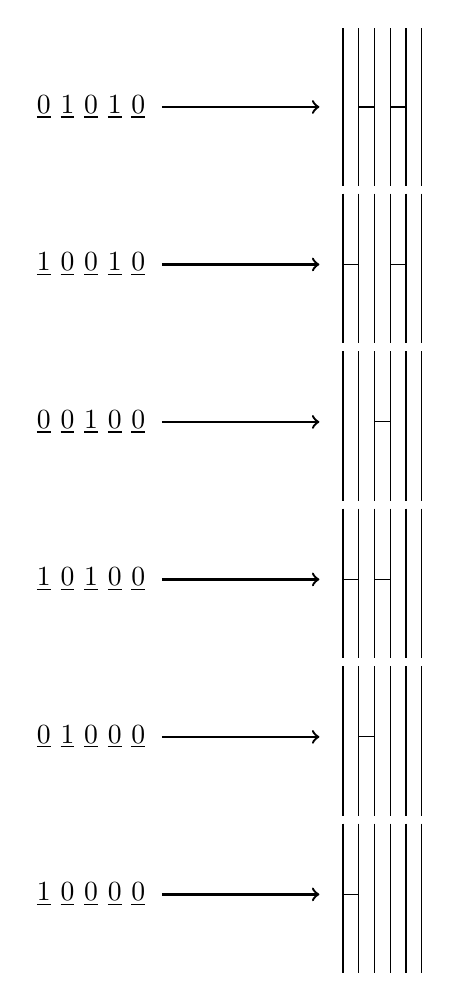
\begin{tikzpicture}
          %%B7
        \node at(0, 0){\underline{$0$}};
        \node at(0.3, 0){\underline{$1$}};
        \node at(0.6, 0){\underline{$0$}};
        \node at(0.9, 0){\underline{$1$}};
        \node at(1.2, 0){\underline{$0$}};
            \draw[->, line width = .3mm](1.5, 0) to (3.5, 0);
        %%L7
        \draw(3.8, -1) to (3.8, 1);
        \draw(4, -1) to (4, 1);
        \draw(4.2, -1) to (4.2, 1);
            \draw(4, 0) to (4.2, 0);
        \draw(4.4, -1) to (4.4, 1);
            \draw(4.4, 0) to (4.6, 0);
        \draw(4.6, -1) to (4.6, 1);
        \draw(4.8, -1) to (4.8, 1);


        %%B8
        \node at(0, -2){\underline{$1$}};
        \node at(0.3, -2){\underline{$0$}};
        \node at(0.6, -2){\underline{$0$}};
        \node at(0.9, -2){\underline{$1$}};
        \node at(1.2, -2){\underline{$0$}};
            \draw[->, line width = .3mm](1.5, -2) to (3.5, -2);
        %%L8
        \draw(3.8, -1.1) to (3.8, -3);
        \draw(4, -1.1) to (4, -3);
        \draw(4.2, -1.1) to (4.2, -3);
            \draw(3.8, -2) to (4, -2);
        \draw(4.4, -1.1) to (4.4, -3);
            \draw(4.4, -2) to (4.6, -2);
        \draw(4.6, -1.1) to (4.6, -3);
        \draw(4.8, -1.1) to (4.8, -3);


         %%B9
        \node at(0, -4){\underline{$0$}};
        \node at(0.3, -4){\underline{$0$}};
        \node at(0.6, -4){\underline{$1$}};
        \node at(0.9, -4){\underline{$0$}};
        \node at(1.2, -4){\underline{$0$}};
            \draw[->, line width = .3mm](1.5, -4) to (3.5, -4);
        %%L9
        \draw(3.8, -3.1) to (3.8, -5);
        \draw(4, -3.1) to (4, -5);
        \draw(4.2, -3.1) to (4.2, -5);
            \draw(4.2, -4) to (4.4, -4);
        \draw(4.4, -3.1) to (4.4, -5);
        \draw(4.6, -3.1) to (4.6, -5);
        \draw(4.8, -3.1) to (4.8, -5);


        
         %%B10
        \node at(0, -6){\underline{$1$}};
        \node at(0.3, -6){\underline{$0$}};
        \node at(0.6, -6){\underline{$1$}};
        \node at(0.9, -6){\underline{$0$}};
        \node at(1.2, -6){\underline{$0$}};
            \draw[->, line width = .3mm](1.5, -6) to (3.5, -6);
        %%L10
        \draw(3.8, -5.1) to (3.8, -7);
            \draw(3.8, -6) to (4,-6);
        \draw(4, -5.1) to (4, -7);
        \draw(4.2, -5.1) to (4.2, -7);
            \draw(4.2, -6) to (4.4, -6);
        \draw(4.4, -5.1) to (4.4, -7);
        \draw(4.6, -5.1) to (4.6, -7);
        \draw(4.8, -5.1) to (4.8, -7);

        %%B1
        \node at(0, -8){\underline{$0$}};
        \node at(0.3, -8){\underline{$1$}};
        \node at(0.6, -8){\underline{$0$}};
        \node at(0.9, -8){\underline{$0$}};
        \node at(1.2, -8){\underline{$0$}};
            \draw[->, line width = .3mm](1.5, -8) to (3.5, -8);
        %%L11
        \draw(3.8, -7.1) to (3.8, -9);
        \draw(4, -7.1) to (4, -9);
            \draw(4, -8) to (4.2, -8);
        \draw(4.2, -7.1) to (4.2, -9);
        \draw(4.4, -7.1) to (4.4, -9);
        \draw(4.6, -7.1) to (4.6, -9);
        \draw(4.8, -7.1) to (4.8, -9);

         %%B12
        \node at(0, -10){\underline{$1$}};
        \node at(0.3, -10){\underline{$0$}};
        \node at(0.6, -10){\underline{$0$}};
        \node at(0.9, -10){\underline{$0$}};
        \node at(1.2, -10){\underline{$0$}};
            \draw[->, line width = .3mm](1.5, -10) to (3.5, -10);
        %%L12
        \draw(3.8, -9.1) to (3.8, -11);
            \draw(3.8, -10) to (4, -10);
        \draw(4, -9.1) to (4, -11);
        \draw(4.2, -9.1) to (4.2, -11);
        \draw(4.4, -9.1) to (4.4, -11);
        \draw(4.6, -9.1) to (4.6, -11);
        \draw(4.8, -9.1) to (4.8, -11);
        \end{tikzpicture}
    \end{minipage}

    \caption{All 12 binary strings of length $5$ with at least one $1$ and no consecutive $1s$ maps to all twelve ladders of order $6$ with a height of one. 
    The recurrence relation being $L(6)=2L(4)+(L(5)-L(4))+1=L(4)+L(5)+1$}
\end{figure}
\end{center}

\subsubsection{Closed form Formula for Ladders of Order $N$ with a Height of One}
Before providing the closed form formula for the number of ladders with a height of one, it is important to connect ladders with a height of one to other 
mathematical phenomena because ladders with a height follow the same pattern as these other mathematical phenomena. These phenomena include 
the number of involutions in the Symmetric Group $S_{N}$, the $Nth$ Fibonacci meander, and the number of allowable transitions rules for passing from 
one change to the next in the English art of bell ringing - insert ref. Each of these other mathematical phenomena will be expained along with their 
connections to ladders of order $N$ with a height of one.\par 

Let $S_{N}$ be a the symmetric group of degree $N$ such that each of its elements are one of the $N!$ permutations of order $N$. Let the group 
operation of $S$ be the composition of two permutations (not necessarily unqique) of order $N-1$. Let an \emph{involution} 
be defined as a composition of a permutation with itself such that the result of the composition is the identity permutation. 
For example, $X=\{1, 2, 3\}$. Let $S_{X} = S_{N} = \{(1,2,3),(1,3,2),(2,1,3),(2,3,1),(3,1,2),(3,2,1)\}$. The involutions of $S_{N}=\{(2,1,3),(1,3,2),(1,2,3)\}$.
The reason these are the involutions is because when we define a permutation as a bijective function on the identity permutation, we can see the the composition 
of a permutation from the involution set with itself returns the identity permutation. Let $(1,2,3)=F$,$(2,1,3)=G$ and $(1,3,2)=H$ then we have $F \circ F=(1,2,3)$,
$G \circ G = (1,2,3)$ and $H \circ H=(1,2,3)$. To see an example of the mapping of the composition of $(2,1,3)$ with itself see figure -- fig.\pagebreak  


\begin{figure}
 \centering
 \begin{tikzpicture}[ele/.style={fill=black,circle,minimum width=.8pt,inner sep=1pt},every fit/.style={ellipse,draw,inner sep=-2pt}]
  \node[ele,label=left:$1$] (a1) at (0,4) {};    
  \node[ele,label=left:$2$] (a2) at (0,3) {};    
  \node[ele,label=left:$3$] (a3) at (0,2) {};

  \node[ele,,label=right:$1$] (b1) at (4,4) {};
  \node[ele,,label=right:$2$] (b2) at (4,3) {};
  \node[ele,,label=right:$3$] (b3) at (4,2) {};

  \node [ele,,label=right:$1$](c1) at (8,4){};
  \node [ele,,label=right:$2$](c2) at (8,3){};
  \node [ele,,label=right:$3$](c3) at (8,2){};
  \node[draw,fit= (a1) (a2) (a3),minimum width=2cm] {} ;
  \node[draw,fit= (b1) (b2) (b3), minimum width=2cm] {} ;  
  \node[draw,fit= (c1) (c2) (c3), minimum width=2cm] {} ;  

  \draw[->,thick,shorten <=2pt,shorten >=2pt] (a1) -- (b2);
  \draw[->,thick,shorten <=2pt,shorten >=2] (a2) -- (b1);
  \draw[->,thick,shorten <=2pt,shorten >=2] (a3) -- (b3);
  \draw[->,thick,shorten <=0pt,shorten >=0pt] (b1) -- (c2);
  \draw[->,thick,shorten <=1pt,shorten >=2pt] (b2) -- (c1);
  \draw[->,thick,shorten <=1pt,shorten >=2pt] (b3) -- (c3);

  \node at (2,4.5){$F(1,2,3)$};
  \node at(6,4.5){$F \circ F(1,2,3)$};
 \end{tikzpicture}
\end{figure}

\begin{theorem}
    There is a surjective function between ladders of order $N$ with a height of one and the involution set of $S_{N}$. Note that 
if one were includes the ladder of order $N$ with a height of zero, then there is a bijective function between ladders of order $N$ with a height of zero or one and the involution set of $S_{N}$.
\end{theorem}
\begin{proof}
    The involution set of $S_{N}$ consists of all permutations of order $N$ such that when composed with themselves, the result of the composition is the identity permutation. 
    If a permutation is an involution it either has no inversions or for each pair of inversions, the inversion pairs are pairwise disjoint. That is to say, no element in the 
    involution forms more than $1$ inversion. When inversion pairs are pairwise disjoint, 
    each element in the pair is rotated by one position from its position in the identity permutation. When an involution is composed with the identity permutation, each element is 
    rotated by one or zero positions. If an element from the identity permutation is rotated two times over over a span of two positions, the element returns to its original position in the identity permutation.
    Thus, composing an involution with itself either rotates an element zero times or it rotates an element twice over a span of two positions, thus placing the element in its 
    original position in the identity permutation.\par 
    A ladder of order $N$ with a height of one consists only of bars such that each bar swaps an element in $\pi$ to its correct position in the identity permutation. Suppose an element, $X$,
    needed to be swappped more than once in $L_{\pi}$ to reach its position in the identity permutation. This would mean the route of $X>1$. If that is the case, then the bars of route $X$ require their own rows, seeing as each bar of an element's route 
    cannot be on the same row as any of the other bars of its route. But if that is the case then we have a contradiction seeing as we supposed ladders of order $N$ with a height of one.
    Then it must be the case that for all ladders of order $N$ with a height of one, each bar in any of these given ladders swaps an elmenet in $\pi$ to its correct position 
    in the idetity permutation. That is to say, every ladder of order $N$ with a height of $1$ sorts a $\pi$ such that each element in $\pi$ forms at most 
    one inversion.
    To see a bijective mapping between ladders of order $5$ with a height of zero or one and the involution set of $S_{5}$ please refer to figure --fig.
\end{proof}\pagebreak

\begin{figure}
    \centering
        \begin{minipage}{.4\textwidth}
            \begin{tikzpicture}
            \draw(0,0) to (0,2);
        \draw(.5,0) to (.5,2);
        \draw(1,0) to (1,2);
        \draw(1.5,0) to (1.5,2);
        \draw(2,0) to (2,2);
    
        \draw[->, line width = .3mm](2.3, 1) to (4.3, 1);

        \node at(4.6, 1){$1$};
        \node at(4.9, 1){$2$};
        \node at(5.2, 1){$3$};
        \node at(5.5, 1){$4$};
        \node at(5.8, 1){$5$};

        \draw(0,3) to (0,5);
        \draw(.5,3) to (.5,5);
        \draw(1,3) to (1,5);
        \draw(1.5,3) to (1.5,5);
            \draw(1.5, 4) to (2,4);
        \draw(2,3) to (2,5);
    
        \draw[->, line width = .3mm](2.3, 4) to (4.3, 4);

        \node at(4.6, 4){$1$};
        \node at(4.9, 4){$2$};
        \node at(5.2, 4){$3$};
        \node at(5.5, 4){$5$};
        \node at(5.8, 4){$4$};

        \draw(0,6) to (0,8);
        \draw(.5,6) to (.5,8);
            \draw(.5, 7) to (1, 7);
        \draw(1,6) to (1,8);
        \draw(1.5,6) to (1.5,8);
            \draw(1.5, 7) to (2,7);
        \draw(2,6) to (2,8);
    
        \draw[->, line width = .3mm](2.3, 7) to (4.3, 7);

        \node at(4.6, 7){$1$};
        \node at(4.9, 7){$3$};
        \node at(5.2, 7){$2$};
        \node at(5.5, 7){$5$};
        \node at(5.8, 7){$4$};

        \draw(0,9) to (0,11);
        \draw(.5,9) to (.5,11);
            \draw(0, 10) to (.5, 10);
        \draw(1,9) to (1,11);
        \draw(1.5,9) to (1.5,11);
            \draw(1.5, 10) to (2,10);
        \draw(2,9) to (2,11);
    
        \draw[->, line width = .3mm](2.3, 10) to (4.3, 10);

        \node at(4.6, 10){$2$};
        \node at(4.9, 10){$1$};
        \node at(5.2, 10){$3$};
        \node at(5.5, 10){$5$};
        \node at(5.8, 10){$4$};
            \end{tikzpicture}
        \end{minipage}
        \begin{minipage}{.4\textwidth}
            \begin{tikzpicture}
            \draw(0,12) to (0,14);
        \draw(.5,12) to (.5,14);
        \draw(1,12) to (1,14);
        \draw(1.5,12) to (1.5,14);
            \draw(1, 13) to (1.5,13);
        \draw(2,12) to (2,14);
    
        \draw[->, line width = .3mm](2.3, 13) to (4.3, 13);

        \node at(4.6, 13){$1$};
        \node at(4.9, 13){$2$};
        \node at(5.2, 13){$4$};
        \node at(5.5, 13){$3$};
        \node at(5.8, 13){$5$};

        \draw(0,15) to (0,17);
            \draw(0, 16) to (0.5, 16);
        \draw(.5,15) to (.5,17);
        \draw(1,15) to (1,17);
        \draw(1.5,15) to (1.5,17);
            \draw(1, 16) to (1.5,16);
        \draw(2,15) to (2,17);
    
        \draw[->, line width = .3mm](2.3, 16) to (4.3, 16);

        \node at(4.6, 16){$2$};
        \node at(4.9, 16){$1$};
        \node at(5.2, 16){$4$};
        \node at(5.5, 16){$3$};
        \node at(5.8, 16){$5$};

        \draw(0,18) to (0,20);
        \draw(.5,18) to (.5,20);
        \draw(1,18) to (1,20);
        \draw(1.5,18) to (1.5,20);
            \draw(.5, 19) to (1,19);
        \draw(2,18) to (2,20);
    
        \draw[->, line width = .3mm](2.3, 19) to (4.3, 19);

        \node at(4.6, 19){$1$};
        \node at(4.9, 19){$3$};
        \node at(5.2, 19){$2$};
        \node at(5.5, 19){$4$};
        \node at(5.8, 19){$5$};

        \draw(0,21) to (0,23);
        \draw(.5,21) to (.5,23);
        \draw(1,21) to (1,23);
        \draw(1.5,21) to (1.5,23);
            \draw(0, 22) to (.5,22);
        \draw(2,21) to (2,23);
    
        \draw[->, line width = .3mm](2.3, 22) to (4.3, 22);

        \node at(4.6, 22){$2$};
        \node at(4.9, 22){$1$};
        \node at(5.2, 22){$3$};
        \node at(5.5, 22){$4$};
        \node at(5.8, 22){$5$};
            \end{tikzpicture}
        \end{minipage}
        
\end{figure}
%%End section with ladders of a height of zero or one